\documentclass[11pt]{article}

\usepackage[margin=2.2cm]{geometry}

\usepackage{longtable,booktabs,multirow,array,amsmath,amssymb}

\usepackage[dvipsnames]{xcolor}

\usepackage{tikz}

\usetikzlibrary{shapes,arrows,arrows.meta,positioning,shapes.geometric,calc,fit}

\usepackage[hidelinks]{hyperref}   % DOIs in the bibliography contain underscores

\providecommand{\prcount}[1]{\mbox{\textit{n}=#1}}

\renewcommand{\thetable}{S\arabic{table}}

\renewcommand{\thefigure}{S\arabic{figure}}

\begin{document}

\begin{center}

{\Large\bfseries Supplementary Material}\\[4pt]

{\large The Metric Blind Spot in Deep Learning-Based Brain MRI Reconstruction: A Systematic Review}

\end{center}

\vspace{8pt}

\noindent Supplementary Tables S1--S3 list all 263 included primary studies in ascending order of publication year within each part (studies 1--110, 111--220 and 221--263). Tables S4--S9 carry the review's methodological detail: the comparison against related secondary studies (S4), the search vocabulary and its derivation (S5), the extraction form (S6), the thematic evidence architecture (S7), the four metric-failure mechanisms with their evidence sources (S8), and the provenance of every released data file (S9). Tables S10--S12 carry the supporting detail for Section 4.5 of the main manuscript: the fastMRI+ annotation-layer derivation (S10), the disjoint-strata correction for the sequence contrast (S11), and the venue cross-tabulation with evaluation-paradigm multiplicity (S12). Full bibliographic details for every included study appear in the reference list at the end of this document; that list is self-contained and does not depend on the main manuscript's references.

\vspace{8pt}

\clearpage

% Longtable version of Supplementary Tables S1-S2 for the elsarticle
% (Computerized Medical Imaging and Graphics) build; generated from supplementary_table_s1.tex.
\clearpage
\setcounter{table}{0}
\renewcommand{\thetable}{S\arabic{table}}

{\def\baselinestretch{1}\scriptsize
\setlength{\tabcolsep}{3pt}
\renewcommand{\arraystretch}{1.06}
\begin{longtable}{r l p{0.27\textwidth} r l p{0.27\textwidth}}
\caption{The 263 primary studies included in the review, ordered by publication year (part 1 of 3: studies 1--110). Per-study extracted characteristics and risk-of-bias ratings for all studies are released as \texttt{included\_characteristics.csv} and \texttt{included\_characteristics\_supplement.csv} (Data and Code Availability).}\label{tab:supp_included_1}\\
\hline
\textbf{\#} & \textbf{Study} & \textbf{Venue (year)} & \textbf{\#} & \textbf{Study} & \textbf{Venue (year)} \\
\hline
\endfirsthead
\multicolumn{6}{l}{\footnotesize\emph{(continued)}}\\
\hline
\textbf{\#} & \textbf{Study} & \textbf{Venue (year)} & \textbf{\#} & \textbf{Study} & \textbf{Venue (year)} \\
\hline
\endhead
\hline
\endfoot
1 & \cite{gardner1995detection} & Academic radiology (1995) & 56 & \cite{duffy2021retrospective} & NeuroImage (2021) \\
2 & \cite{cao1995using} & IEEE Transactions on Medical Imaging (1995) & 57 & \cite{kim2021simultaneous} & Tomography (Ann Arbor, Mich.) (2021) \\
3 & \cite{fadeev2005quality} & Proceedings of the Fifth IEEE International Symposium on Signal Processing and Information Technology, 2005. (2005) & 58 & \cite{gao2021xqsm} & NMR in biomedicine (2021) \\
4 & \cite{tisdall2006using} & IEEE transactions on medical imaging (2006) & 59 & \cite{kulkarni2021dictionary} & IEEE Open Journal of Signal Processing (2021) \\
5 & \cite{miao2010comprehensive} & SPIE Proceedings (2010) & 60 & \cite{tanno2021uncertainty} & NeuroImage (2021) \\
6 & \cite{miao2013a} & Magnetic resonance imaging (2013) & 61 & \cite{karimi2021accurate} & MICCAI 2021, LNCS 12907 (2021) \\
7 & \cite{li2015artifactual} & Journal of magnetic resonance imaging : JMRI (2015) & 62 & \cite{garmaoehmichen2021evaluation} & 2021 43rd Annual International Conference of the IEEE Engineering in Medicine \& Biology Society (EMBC) (2021) \\
8 & \cite{ning2015sparse} & Medical image analysis (2015) & 63 & \cite{kumar2021learning} & 2021 43rd Annual International Conference of the IEEE Engineering in Medicine \& Biology Society (EMBC) (2021) \\
9 & \cite{elhabian2016compressive} & 2016 IEEE 13th International Symposium on Biomedical Imaging (ISBI) (2016) & 64 & \cite{zhang2022a} & NeuroImage (2022) \\
10 & \cite{lacerda2016diffusion} & Magnetic resonance in medicine (2016) & 65 & \cite{zibetti2022alternating} & IEEE Transactions on Computational Imaging (2022) \\
11 & \cite{zahneisen2016reverse} & Magnetic resonance in medicine (2016) & 66 & \cite{conklin2022clinical} & European radiology (2022) \\
12 & \cite{kayvanrad2016diagnostic} & Journal of Magnetic Resonance Imaging (2016) & 67 & \cite{sheng2022deep} & Contrast media \& molecular imaging (2022) \\
13 & \cite{esteban2017mriqc} & PloS one (2017) & 68 & \cite{huang2022deep} & Nan fang yi ke da xue xue bao = Journal of Southern Medical University (2022) \\
14 & \cite{kim2017artificial} & Magnetic Resonance Imaging (2017) & 69 & \cite{begnoche2022epi} & Magnetic resonance imaging (2022) \\
15 & \cite{chow2017modifiedbrisque} & Magnetic Resonance Imaging (2017) & 70 & \cite{radmanesh2022exploring} & Radiology. Artificial intelligence (2022) \\
16 & \cite{yu2018a} & BMC medical imaging (2018) & 71 & \cite{sannananja2022imagequality} & AJNR. American journal of neuroradiology (2022) \\
17 & \cite{gurbani2018a} & Magnetic resonance in medicine (2018) & 72 & \cite{yasaka2022impact} & Japanese journal of radiology (2022) \\
18 & \cite{fantini2018automatic} & 2018 International Workshop on Pattern Recognition in Neuroimaging (PRNI) (2018) & 73 & \cite{muro2022improvement} & Nihon Hoshasen Gijutsu Gakkai zasshi (2022) \\
19 & \cite{osadebey2018blind} & Biomedical engineering online (2018) & 74 & \cite{pirkl2022learning} & Medical image analysis (2022) \\
20 & \cite{risk2018impacts} & NeuroImage (2018) & 75 & \cite{yang2022modelbased} & IEEE transactions on medical imaging (2022) \\
21 & \cite{gong2018deep} & Journal of Magnetic Resonance Imaging (2018) & 76 & \cite{ma2022mitigating} & Magnetic resonance in medicine (2022) \\
22 & \cite{tang2019accelerated} & Korean journal of radiology (2019) & 77 & \cite{yoshida2022motion} & PloS one (2022) \\
23 & \cite{zhao2019applications} & Magnetic resonance imaging (2019) & 78 & \cite{g2022quantitative} & NMR in Biomedicine (2022) \\
24 & \cite{sujit2019automated} & Journal of magnetic resonance imaging : JMRI (2019) & 79 & \cite{srikant2022quantitative} & Scientific Reports (2022) \\
25 & \cite{vranic2019compressed} & AJNR. American journal of neuroradiology (2019) & 80 & \cite{sui2022scanspecific} & IEEE Transactions on Medical Imaging (2022) \\
26 & \cite{glessgen2019evaluation} & Neuroradiology (2019) & 81 & \cite{hu2022spatiotemporal} & IEEE transactions on bio-medical engineering (2022) \\
27 & \cite{hagiwara2019improving} & AJNR. American journal of neuroradiology (2019) & 82 & \cite{pawar2022suppressing} & NMR in biomedicine (2022) \\
28 & \cite{haskell2019network} & Magnetic resonance in medicine (2019) & 83 & \cite{qiao2022unsupervised} & IEEE transactions on medical imaging (2022) \\
29 & \cite{bollmann2019sharqnet} & Zeitschrift fur medizinische Physik (2019) & 84 & \cite{almasni2022stacked} & NeuroImage (2022) \\
30 & \cite{elsaid2019superresolution} & Annual International Conference of the IEEE Engineering in Medicine and Biology Society. IEEE Engineering in Medicine and Biology Society. Annual International Conference (2019) & 85 & \cite{kanemaru2022effect} & Journal of neuroradiology = Journal de neuroradiologie (2022) \\
31 & \cite{ryu2019data} & Journal of magnetic resonance imaging : JMRI (2019) & 86 & \cite{kim2022deep} & Neuroradiology (2022) \\
32 & \cite{delattre2019compressed} & European Radiology (2019) & 87 & \cite{chan2022signal} & Magnetic Resonance in Medicine (2022) \\
33 & \cite{zhang2019mri} & Magnetic Resonance in Medicine (2019) & 88 & \cite{song2022jointly} & Journal of Magnetic Resonance (2022) \\
34 & \cite{zhang2019robust} & IEEE Transactions on Medical Imaging (2019) & 89 & \cite{wismuller2022selfsupervised} & Real-Time Image Processing and Deep Learning 2022 (2022) \\
35 & \cite{sommer2020correction} & AJNR. American journal of neuroradiology (2020) & 90 & \cite{gngr2023adaptive} & Medical image analysis (2023) \\
36 & \cite{benjamin2020diagnostic} & Magnetic resonance imaging (2020) & 91 & \cite{lang2023clinical} & AJNR. American journal of neuroradiology (2023) \\
37 & \cite{hampe2020investigating} & Physics in medicine and biology (2020) & 92 & \cite{johannes2023comparison} & Clinical Neuroradiology (2023) \\
38 & \cite{vanderhasselt2020synthetic} & AJNR. American journal of neuroradiology (2020) & 93 & \cite{chen2023ddcisenet} & arXiv.org (2023) \\
39 & \cite{du2020brain} & IEEE Access (2020) & 94 & \cite{pizarro2023deep} & Medical image analysis (2023) \\
40 & \cite{hales2020combined} & Journal of magnetic resonance imaging : JMRI (2020) & 95 & \cite{hossbach2023deep} & Medical physics (2023) \\
41 & \cite{chung2020restoration} & IEEE Signal Processing Letters (2020) & 96 & \cite{li2023diffusion} & Medical image analysis (2023) \\
42 & \cite{liu2020motion} & Magnetic Resonance Imaging (2020) & 97 & \cite{shan2023distortioncorrected} & Magnetic resonance in medicine (2023) \\
43 & \cite{wang2020synthesize} & IEEE Transactions on Medical Imaging (2020) & 98 & \cite{thaler2023effect} & PloS one (2023) \\
44 & \cite{meng2020accelerating} & Magnetic Resonance in Medicine (2021) & 99 & \cite{usui2023evaluation} & Scientific reports (2023) \\
45 & \cite{zhang2021apiremc} & Magnetic resonance imaging (2021) & 100 & \cite{ciceri2023geometric} & Neuroinformatics (2023) \\
46 & \cite{ding2021acceleration} & AJNR. American journal of neuroradiology (2021) & 101 & \cite{ramosllordn2023highfidelity} & NMR in biomedicine (2023) \\
47 & \cite{harper2021assessing} & NeuroImage. Clinical (2021) & 102 & \cite{ji2023highly} & Magnetic resonance in medicine (2023) \\
48 & \cite{duong2021correcting} & Sensors (Basel, Switzerland) (2021) & 103 & \cite{simk2023improving} & BMC medical imaging (2023) \\
49 & \cite{bash2021deep} & AJNR. American journal of neuroradiology (2021) & 104 & \cite{jiang2023multimodal} & Journal of digital imaging (2023) \\
50 & \cite{sagawa2021deep} & Magnetic resonance in medical sciences : MRMS : an official journal of Japan Society of Magnetic Resonance in Medicine (2021) & 105 & \cite{tabari2023optimized} & European radiology experimental (2023) \\
51 & \cite{kwan2021deep} & Scientific Reports (2021) & 106 & \cite{nivetha2023sadir} & Shape in Medical Imaging (2023) \\
52 & \cite{karimi2021deep} & NeuroImage (2021) & 107 & \cite{yilmaz2023selfsupervised} & Medical Image Computing and Computer Assisted Intervention – MICCAI 2023 (2023) \\
53 & \cite{dieckmeyer2021effect} & Magma (New York, N.Y.) (2021) & 108 & \cite{wang2023spatialintensity} & IEEE transactions on medical imaging (2023) \\
54 & \cite{hu2021runup} & Magnetic resonance in medicine (2021) & 109 & \cite{vakli2023automatic} & Medical image analysis (2023) \\
55 & \cite{muckley2021results} & IEEE Transactions on Medical Imaging (2021) & 110 & \cite{corderogrande2023fetal} & IEEE Transactions on Medical Imaging (2023) \\
\hline
\end{longtable}}

{\def\baselinestretch{1}\scriptsize
\setlength{\tabcolsep}{3pt}
\renewcommand{\arraystretch}{1.06}
\begin{longtable}{r l p{0.27\textwidth} r l p{0.27\textwidth}}
\caption{The 263 primary studies included in the review, ordered by publication year (part 2 of 3: studies 111--220).}\label{tab:supp_included_2}\\
\hline
\textbf{\#} & \textbf{Study} & \textbf{Venue (year)} & \textbf{\#} & \textbf{Study} & \textbf{Venue (year)} \\
\hline
\endfirsthead
\multicolumn{6}{l}{\footnotesize\emph{(continued)}}\\
\hline
\textbf{\#} & \textbf{Study} & \textbf{Venue (year)} & \textbf{\#} & \textbf{Study} & \textbf{Venue (year)} \\
\hline
\endhead
\hline
\endfoot
111 & \cite{zhou2023mitigating} & Physics in medicine and biology (2023) & 166 & \cite{yoo2025evaluation} & Korean journal of radiology (2025) \\
112 & \cite{lau2023pushing} & Magnetic resonance in medicine (2023) & 167 & \cite{tang2025incorporating} & Journal of magnetic resonance imaging : JMRI (2025) \\
113 & \cite{ernst2023sinogram} & Neural networks : the official journal of the International Neural Network Society (2023) & 168 & \cite{nimje2025insights} & NMR in biomedicine (2025) \\
114 & \cite{matsuo2023feasibility} & Neuroradiology (2023) & 169 & \cite{mercier2025intersectionbased} & Computers in biology and medicine (2025) \\
115 & \cite{beljaards2024aibased} & Medical physics (2024) & 170 & \cite{singh2025learningbased} & Magnetic resonance in medicine (2025) \\
116 & \cite{i2024accelerated} & Scientific Reports (2024) & 171 & \cite{raymond2025leveraging} & AJNR. American journal of neuroradiology (2025) \\
117 & \cite{zhou2024adversarial} & IEEE Access (2024) & 172 & \cite{taymourtash2025measuring} & Human brain mapping (2025) \\
118 & \cite{dolui2024automated} & Journal of magnetic resonance imaging : JMRI (2024) & 173 & \cite{karuna2025modified} & Scientific reports (2025) \\
119 & \cite{heo2024cest} & Magnetic resonance in medicine (2024) & 174 & \cite{goffi2025multimetric} & Human brain mapping (2025) \\
120 & \cite{lang2024ultrafast} & American Journal of Neuroradiology (2024) & 175 & \cite{byanju2025myelin} & Magma (New York, N.Y.) (2025) \\
121 & \cite{karthik2024comprehensive} & BMC medical imaging (2024) & 176 & \cite{karl2025nonreference} & Deep Generative Models (2025) \\
122 & \cite{lee2024deep} & Scientific reports (2024) & 177 & \cite{chen2025pwgan} & bioRxiv (2025) \\
123 & \cite{uher2024deepflair} & Magnetic resonance imaging (2024) & 178 & \cite{li2025patientspecific} & Physics in medicine and biology (2025) \\
124 & \cite{bian2024improving} & Magnetic resonance in medicine (2024) & 179 & \cite{sepideh2025probabilistic} & Scientific Reports (2025) \\
125 & \cite{yasaka2024iterative} & Journal of imaging informatics in medicine (2024) & 180 & \cite{choi2025prospective} & Korean journal of radiology (2025) \\
126 & \cite{trivedi2024mcddpm} & 2024 17th International Congress on Image and Signal Processing, BioMedical Engineering and Informatics (CISP-BMEI) (2024) & 181 & \cite{jochmann2025quantitative} & Magnetic resonance in medicine (2025) \\
127 & \cite{ma2024mri} & BMC medical imaging (2024) & 182 & \cite{wichtmann2025rapid} & Pediatric radiology (2025) \\
128 & \cite{khawaled2024npbrec} & Artificial intelligence in medicine (2024) & 183 & \cite{wang2025rapid} & Magnetic resonance in medicine (2025) \\
129 & \cite{kofler2024quantitative} & IEEE Transactions on Biomedical Engineering (2024) & 184 & \cite{verdicchio2025reliability} & Scientific reports (2025) \\
130 & \cite{gil2024quantitative} & NeuroImage (2024) & 185 & \cite{jung2025reliability} & Neuroradiology (2025) \\
131 & \cite{qiu2024selfcalibrated} & Magnetic resonance in medicine (2024) & 186 & \cite{safari2025resmocodiff} & Physics in medicine and biology (2025) \\
132 & \cite{olsson2024simulating} & PloS one (2024) & 187 & \cite{aali2025robust} & Magnetic resonance in medicine (2025) \\
133 & \cite{rizzuti2024towards} & Magma (New York, N.Y.) (2024) & 188 & \cite{dong2025romerepti} & Magnetic resonance in medicine (2025) \\
134 & \cite{altmann2024ultrafast} & Radiology (2024) & 189 & \cite{dabrowski2025sismik} & IEEE transactions on medical imaging (2025) \\
135 & \cite{jun2024zerodeepsub} & Magnetic resonance in medicine (2024) & 190 & \cite{huber2025shortterm} & Magnetic resonance in medicine (2025) \\
136 & \cite{yuan2024novel} & Medical physics (2024) & 191 & \cite{alalar2025sparsitydriven} & 2025 IEEE International Conference on Image Processing (ICIP) (2025) \\
137 & \cite{wada2024deep} & Journal of magnetic resonance imaging : JMRI (2024) & 192 & \cite{wang2025spherical} & Magnetic resonance in medicine (2025) \\
138 & \cite{hewlett2024deep} & NMR in biomedicine (2024) & 193 & \cite{dewey2025superresolution} & AJNR. American journal of neuroradiology (2025) \\
139 & \cite{xie2024based} & Medical physics (2024) & 194 & \cite{liu2025timeefficient} & Magnetic resonance in medicine (2025) \\
140 & \cite{moshe2024handling} & Journal of magnetic resonance imaging : JMRI (2024) & 195 & \cite{bauman2025ultrahighresolution} & Zeitschrift fur medizinische Physik (2025) \\
141 & \cite{desalegn2024hara} & IEEE Access (2024) & 196 & \cite{muro2025using} & Magnetic resonance in medical sciences : MRMS : an official journal of Japan Society of Magnetic Resonance in Medicine (2025) \\
142 & \cite{yarach2024reconstruction} & Magnetic Resonance Materials in Physics, Biology and Medicine (2024) & 197 & \cite{wang2025variableflipangle} & Magnetic resonance in medicine (2025) \\
143 & \cite{shan2024image} & IEEE Transactions on Instrumentation and Measurement (2024) & 198 & \cite{rauland2025white} & Human brain mapping (2025) \\
144 & \cite{ismail2024performance} & 2024 3rd International Conference on Creative Communication and Innovative Technology (ICCIT) (2024) & 199 & \cite{wu2025application} & Journal of magnetic resonance imaging : JMRI (2025) \\
145 & \cite{milovic2024xsim} & Magnetic Resonance in Medicine (2025) & 200 & \cite{sakitis2025bayesian} & Magnetic resonance imaging (2025) \\
146 & \cite{feizollah2025d} & Magnetic resonance in medicine (2025) & 201 & \cite{brunatova2025denoising} & Magnetic resonance in medicine (2025) \\
147 & \cite{won2025a} & Scientific Reports (2025) & 202 & \cite{lan2025diffusion} & NeuroImage (2025) \\
148 & \cite{safari2025a} & Medical physics (2025) & 203 & \cite{huijben2025enhancing} & Computer methods and programs in biomedicine (2025) \\
149 & \cite{zhu2025a} & Magnetic resonance in medicine (2025) & 204 & \cite{behrendt2025guided} & Computers in biology and medicine (2025) \\
150 & \cite{nishioka2025accelerating} & Japanese journal of radiology (2025) & 205 & \cite{park2025higher} & Magnetic resonance in medicine (2025) \\
151 & \cite{wen2025accelerating} & BMC medical imaging (2025) & 206 & \cite{meng2025motion} & Magnetic resonance in medicine (2025) \\
152 & \cite{marchetto2025agreement} & Magma (New York, N.Y.) (2025) & 207 & \cite{li2025quantitative} & Medical physics (2025) \\
153 & \cite{liu2025application} & AJNR. American journal of neuroradiology (2025) & 208 & \cite{nagaraj2025slice} & AJNR. American journal of neuroradiology (2025) \\
154 & \cite{bjrkeli2025artificial} & The Journal of international medical research (2025) & 209 & \cite{chen2025mri} & IEEE Transactions on Medical Imaging (2025) \\
155 & \cite{angella2025assessing} & 2025 IEEE 22nd International Symposium on Biomedical Imaging (ISBI) (2025) & 210 & \cite{wu2025d} & IEEE Journal of Biomedical and Health Informatics (2025) \\
156 & \cite{nonninger2025assessment} & European journal of radiology (2025) & 211 & \cite{choi2025accelerated} & Pediatric Radiology (2025) \\
157 & \cite{hosseini2025autocornn} & Journal of imaging informatics in medicine (2025) & 212 & \cite{joshi2025arterial} & 2025 IEEE International Conference on Electronics, Computing and Communication Technologies (CONECCT) (2025) \\
158 & \cite{yarach2025blipup} & Magnetic resonance imaging (2025) & 213 & \cite{liu2025deep} & American Journal of Neuroradiology (2025) \\
159 & \cite{you2025conditional} & NeuroImage (2025) & 214 & \cite{mohsen2025deep} & 2025 Twelfth International Conference on Intelligent Computing and Information Systems (ICICIS) (2025) \\
160 & \cite{zhu2025cycleconditional} & Medical image analysis (2025) & 215 & \cite{xu2025deism} & IEEE Transactions on Biomedical Engineering (2025) \\
161 & \cite{kharaji2025dantecaipi} & AJNR. American journal of neuroradiology (2025) & 216 & \cite{wang2025estimating} & ICONIP 2024, CCIS 2285 (2025) \\
162 & \cite{angella2025dima} & IEEE Access (2025) & 217 & \cite{nagaraj2025evaluation} & Magnetic Resonance Imaging (2025) \\
163 & \cite{liebrand2025deep} & Magma (New York, N.Y.) (2025) & 218 & \cite{takada2025impact} & European Journal of Radiology (2025) \\
164 & \cite{giulio2025diffusion} & Journal of Medical Systems (2025) & 219 & \cite{huang2025improve} & Journal of Magnetic Resonance (2025) \\
165 & \cite{cerjanic2025elastographic} & Magnetic resonance in medicine (2025) & 220 & \cite{harada2025verification} & Magnetic Resonance Imaging (2025) \\
\hline
\end{longtable}}

{\def\baselinestretch{1}\scriptsize
\setlength{\tabcolsep}{3pt}
\renewcommand{\arraystretch}{1.06}
\begin{longtable}{r l p{0.27\textwidth} r l p{0.27\textwidth}}
\caption{The 263 primary studies included in the review, ordered by publication year (part 3 of 3: studies 221--263). Per-study extracted characteristics and methodological quality ratings for all studies are released as \texttt{included\_characteristics.csv} and \texttt{included\_characteristics\_supplement.csv} (Data and Code Availability).}\label{tab:supp_included_3}\\
\hline
\textbf{\#} & \textbf{Study} & \textbf{Venue (year)} & \textbf{\#} & \textbf{Study} & \textbf{Venue (year)} \\
\hline
\endfirsthead
\multicolumn{6}{l}{\footnotesize\emph{(continued)}}\\
\hline
\textbf{\#} & \textbf{Study} & \textbf{Venue (year)} & \textbf{\#} & \textbf{Study} & \textbf{Venue (year)} \\
\hline
\endhead
\hline
\endfoot
221 & \cite{bathla2025deeplearning} & American Journal of Neuroradiology (2026) & 243 & \cite{abed2026mriqt} & 2026 IEEE 23rd International Symposium on Biomedical Imaging (ISBI) (2026) \\
222 & \cite{fujita2025motioninformed} & American Journal of Neuroradiology (2026) & 244 & \cite{ortizgonzalez2026motiondps} & IEEE Transactions on Medical Imaging (2026) \\
223 & \cite{huabing2026accelerating} & Communications Engineering (2026) & 245 & \cite{shen2026realdeal} & Deep Generative Models (2026) \\
224 & \cite{xiong2026advancing} & Magnetic resonance in medicine (2026) & 246 & \cite{rassmann2026regression} & IEEE transactions on medical imaging (2026) \\
225 & \cite{schauman2026an} & Magnetic resonance in medicine (2026) & 247 & \cite{f2026simulationbased} & Communications Medicine (2026) \\
226 & \cite{thomas2026automatic} & Perinatal, Preterm and Paediatric Image Analysis (2026) & 248 & \cite{islam2026synpoc} & Scientific reports (2026) \\
227 & \cite{liu2026blockinterleaved} & Magnetic resonance in medicine (2026) & 249 & \cite{sebastian2026ultrafast} & Clinical Neuroradiology (2026) \\
228 & \cite{lee2026cartesian} & Magnetic resonance in medicine (2026) & 250 & \cite{kim2026vessel} & Magnetic resonance in medicine (2026) \\
229 & \cite{okell2026combined} & Magnetic resonance in medicine (2026) & 251 & \cite{salem2026bald} & Cluster Computing (2026) \\
230 & \cite{marchetto2026contrastoptimized} & Magnetic resonance in medicine (2026) & 252 & \cite{starck2026diff} & IEEE transactions on medical imaging (2026) \\
231 & \cite{beljaards2026deepdisorder} & NMR in biomedicine (2026) & 253 & \cite{saeed2026improved} & Magnetic resonance imaging (2026) \\
232 & \cite{yoshida2026deep} & Scientific reports (2026) & 254 & \cite{liang2026itermask} & Medical image analysis (2026) \\
233 & \cite{baz2026deep} & European radiology (2026) & 255 & \cite{mirza2026learning} & IEEE Transactions on Medical Imaging (2026) \\
234 & \cite{s2026evaluating} & Frontiers in Neuroscience (2026) & 256 & \cite{seonghyeon2026simulation} & MAGNETOCHEMISTRY (2026) \\
235 & \cite{ho2026evaluation} & Journal of magnetic resonance imaging : JMRI (2026) & 257 & \cite{tessema2026technical} & IEEE Access (2026) \\
236 & \cite{mello2026fast} & Scientific reports (2026) & 258 & \cite{xia2026accurate} & European Journal of Radiology (2026) \\
237 & \cite{li2026fewshot} & Magnetic resonance in medicine (2026) & 259 & \cite{solak2026braingan} & Journal of Imaging Informatics in Medicine (2026) \\
238 & \cite{b2026ganbased} & Biomimetics (2026) & 260 & \cite{tabari2026clinical} & American Journal of Neuroradiology (2026) \\
239 & \cite{liu2026highly} & IEEE Transactions on Medical Imaging (2026) & 261 & \cite{jayadeepthi2026deep} & 2026 4th International Conference on Inventive Computing and Informatics (ICICI) (2026) \\
240 & \cite{zhang2026iterative} & Medical image analysis (2026) & 262 & \cite{verclytte2026deep} & American Journal of Neuroradiology (2026) \\
241 & \cite{wei2026latent} & Deep Generative Models (2026) & 263 & \cite{cao2026loddpm} & Biomedical Signal Processing and Control (2026) \\
242 & \cite{junhyeok2026lesionaware} & Medical Image Computing and Computer Assisted Intervention – MICCAI 2025 (2026) & & & \\
\end{longtable}}



\clearpage

\begin{table}[t]
\centering
\caption{Selected secondary studies grouped by academic strand and their key methodological limitations relative to this review.}
\label{tab:related}
\small
\setlength{\tabcolsep}{4pt}
\renewcommand{\arraystretch}{1.15}

\begin{tabular}{
    p{0.24\textwidth}
    p{0.34\textwidth}
    p{0.36\textwidth}
}
\hline
\textbf{Academic Strand} &
\textbf{Scope \& Foundational Focus} &
\textbf{Key Methodological Limitations} \\
\hline

Deep Learning MRI Reconstruction Methods \& Surveys \cite{liang2020deep,montalt2021machine,knoll2020fastmri,kazerouni2023diffusion,gngr2023adaptive,nimje2025insights,liu2026highly}
&
Reconstruction architectures (unrolled physics-based networks, GANs, diffusion priors), acceleration factors, and $k$-space undersampling.
&
Emphasize reconstruction accuracy and efficiency; treat safety, artifacts, and failure modes as secondary and do not systematically map them to evaluation practice.
\\
\hline

Task-Based Image Quality Assessment \cite{barrett1993model,barrett2004foundations,icru54}
&
Objective assessment of image quality by task performance; ideal, Hotelling, and channelized model observers; figures of merit tied to a stated diagnostic task rather than to pixel agreement.
&
Not a limitation of this strand but of its uptake: it established the inadequacy of pixel-wise fidelity for task assessment three decades ago, yet is largely absent from the reconstruction literature reviewed here: no included study evaluated a model observer, and only 57 of 263 carried any reader assessment at all (the verified reader subset; four of the 61 originally labelled were reclassified as algorithmic at appraisal). Documenting that absence, and what follows from it, is one of this review's contributions.
\\
\hline

Image-Quality Metrics \& Observer / Reader Studies \cite{mason2020comparison,tang2025incorporating,yu2018a,muckley2021results,bash2021deep}
&
Pixel-wise (PSNR, SSIM, NRMSE) and perceptual/learned metrics; radiologist rankings and prospective multi-reader diagnostic studies.
&
Establish that pixel-wise metrics agree only weakly with radiologist judgement, but are typically single-study and not synthesized across the reconstruction-safety literature.
\\
\hline

Artifact Detection, Motion Correction \& Robustness \cite{esteban2017mriqc,fantini2018automatic,sommer2020correction,beljaards2024aibased,khawaled2024npbrec}
&
Automated quality-control and artifact/motion detection, motion-correction networks, uncertainty estimation, and out-of-distribution robustness.
&
Address individual failure modes in isolation; no synthesis relates them to reconstruction method families or to downstream diagnostic evaluation.
\\
\hline

Hallucination Analysis in Tomographic Reconstruction \cite{bhadra2021hallucinations,gottschling2020troublesome}
&
Decomposition of reconstruction error into measurement-space and null-space components; hallucination maps isolating prior-induced structure; benchmark bias arising from misuse of processed public data.
&
Establish the null-space account of hallucination and the detection tooling that follows from it, but do not connect it to counterfactual attribution or to review-level evidence on evaluation practice.
\\
\hline

Causal \& Counterfactual Medical-Image Safety \cite{pawlowski2020deep,castro2020causality,sanchez2022healthy,wei2026latent}
&
Structural causal models and counterfactual image synthesis for medical AI, including recent 3D brain MRI counterfactuals.
&
Focus on downstream classification, segmentation, or synthesis; rarely applied to physics-constrained $k$-space reconstruction, and absent from most of the reconstruction-safety studies reviewed here.
\\
\hline
\end{tabular}
\end{table}

\begin{table}[t]
\centering
\caption{Derivation of search vocabulary, MeSH headings, and representative database Boolean query syntax.}
\label{tab:keywords}
\small
\setlength{\tabcolsep}{4pt}
\renewcommand{\arraystretch}{1.18}
\begin{tabular}{>{\raggedright\arraybackslash}p{0.20\textwidth} >{\raggedright\arraybackslash}p{0.34\textwidth} >{\raggedright\arraybackslash}p{0.40\textwidth}}
\hline
\textbf{Conceptual Block} & \textbf{MeSH Headings \& Major Descriptors} & \textbf{Free-Text Keywords, Wildcards \& Boolean Query Syntax} \\
\hline
\textbf{B1.} Neuroimaging Domain \newline \emph{(required)} & \texttt{"Brain"[Mesh]}, \texttt{"Magnetic Resonance Imaging"[Mesh]}, \texttt{"Neuroimaging"[Mesh]} & \texttt{"brain MRI"}, \texttt{"brain magnetic resonance imaging"}, \texttt{"cerebral MRI"}, \texttt{"cranial MRI"}, \texttt{neuroimag*}, \texttt{"brain imaging"}, \texttt{brain scan*}, \texttt{DWI}, \texttt{FLAIR}, \texttt{T1w}, \texttt{T2w}, \texttt{SWI} \\
\hline
\textbf{B2.} AI \& Accelerated Reconstruction \newline \emph{(required)} & \texttt{"Image Processing, Computer-Assisted"[Mesh]}, \texttt{"Deep Learning"[Mesh]}, \texttt{"Machine Learning"[Mesh]} & \texttt{image reconstruction*}, \texttt{"MRI reconstruction"}, \texttt{"accelerated MRI"}, \texttt{"undersampled reconstruction"}, \texttt{"k-space reconstruction"}, \texttt{"deep learning reconstruction"}, \texttt{"unrolled network"}, \texttt{"MoDL"}, \texttt{"GAN"}, \texttt{"diffusion prior"}, \texttt{"Mamba"}, \texttt{"INR"} \\
\hline
\textbf{B3.} Safety, Artifacts \& Evaluation \newline \emph{(required)} & \texttt{"Artifacts"[Mesh]}, \texttt{"Reproducibility of Results"[Mesh]}, \texttt{"Diagnostic Errors"[Mesh]} & \texttt{hallucinat*}, \texttt{"pathology erasure"}, \texttt{"lesion suppression"}, \texttt{reconstruction artifact*}, \texttt{reconstruction error*}, \texttt{"safety evaluation"}, \texttt{"PSNR"}, \texttt{"SSIM"}, \texttt{"metric divergence"}, \texttt{"reader study"}, \texttt{"counterfactual"}, \texttt{"causal auditing"} \\
\hline
\textbf{B4.} Language-Model Observers \newline \emph{(documented prior scoping)} & \texttt{"Natural Language Processing"[Mesh]} & \texttt{LLM*}, \texttt{large language model*}, \texttt{vision-language model*}, \texttt{multimodal large language model*}. Documented during initial protocol scoping; omitted from core database queries to maximize search recall \\
\hline
\multicolumn{3}{p{0.96\textwidth}}{\textbf{X. Exclusion Block} (applied as \texttt{NOT} across digital databases): \texttt{"animal model"}, \texttt{"case report"}, \texttt{"in vitro"}. No publication date limit was applied.} \\
\hline
\multicolumn{3}{p{0.96\textwidth}}{\footnotesize The executed retrieval query in each database combines \texttt{(Block B1) AND (Block B2) AND (Block B3) NOT (Block X)}. the corresponding table of the main manuscript documents the exact executed syntax, fields searched, and hit counts per database. Full search strategy files are open-sourced in the project repository.} \\
\hline
\end{tabular}
\end{table}





\begin{table}[t]
\centering
\caption{(S6) The extraction form as executed, and how each field feeds the synthesis.
Fields are listed in the order they appear in \texttt{included\_characteristics.csv}. The
\emph{basis} column states the text each field was assigned from, because the review's
prevalence counts are floors on what studies report at that basis rather than measurements
of what they did: the screening-level fields were assigned from title, abstract and
controlled vocabulary against the vocabulary fixed in advance (Table~S5), even where full
text was available. Every assigned value carries a verbatim supporting quotation in the
released file. No field was inferred: a variable not stated in the source was recorded as
\emph{not reported}.}
\label{tab:extraction}
\small
\setlength{\tabcolsep}{5pt}
\renewcommand{\arraystretch}{1.15}
\begin{tabular}{p{0.24\textwidth} p{0.20\textwidth} p{0.20\textwidth} p{0.24\textwidth}}
\hline
\textbf{Extracted field} & \textbf{Basis} & \textbf{Appraisal instrument} & \textbf{Feeds} \\
\hline
Method family (compressed sensing / parallel imaging, generative, motion correction,
physics-based unrolled, denoising, super-resolution, self-supervised); multi-label
& Title, abstract, controlled vocabulary
& --- (descriptive)
& Corpus characteristics; the per-family hallucination and reader shares \\
\hline
Evaluation paradigm (pixel-wise, observer/reader, uncertainty, learned/perceptual);
multi-label
& Title, abstract, controlled vocabulary
& --- (descriptive)
& RQ1: the $18/263$ metric--reader co-reporting count and every prevalence share derived
from it \\
\hline
Reported failure modes (artifacts, hallucination or fidelity instability, robustness or
distribution shift); multi-label
& Title, abstract, controlled vocabulary
& --- (descriptive)
& RQ1 and the requirement R4 evidence base \\
\hline
Pulse sequence; field strength; reference standard
& Title, abstract and controlled vocabulary, supplemented from full text for field
strength and sequence where available
& Reporting transparency assessed descriptively against STARD principles
\cite{bossuyt2015stard}
& Corpus characteristics; the disjoint-strata sequence contrast (Table~S11); requirement R3 \\
\hline
Reproducibility indicators (code availability, named public dataset or benchmark, fully
sampled reference, robustness reported)
& Full text where obtainable
& Reproducibility and robustness appraisal, applied to the 206 algorithmic studies
& The code-by-reader cross-tabulation (Table~S12) and the two-communities analysis \\
\hline
Study design (reader/diagnostic vs algorithmic), verified against full text
& Full text; three-reviewer verification
& QUADAS-2 across its four risk-of-bias and three applicability domains
\cite{whiting2011quadas}, applied to the 57 verified reader studies
& The 57/206 partition; all QUADAS-2 tallies; the measured $4/61$ extraction error rate \\
\hline
Acceleration factor $R$ (post-hoc, added after the registered extraction round)
& Full text of all 263 studies, with a verbatim quotation for every value
& --- (descriptive)
& Evaluation practice by acceleration band (main manuscript) \\
\hline
\end{tabular}

\vspace{2pt}
{\footnotesize Two fields the protocol did \emph{not} carry are worth naming, because a
reader may expect them. No metric--reader rank correlation was extracted, since no included
study reports one. No lesion-erasure or hallucination \emph{rate} was extracted; the figures
in the main manuscript's mechanism table are computed from the stated error model, not
measured in any primary study. The auditing framework these requirements motivate is
developed and evaluated in companion work and is outside the scope of this review.}
\end{table}

\begin{table}[t]
\centering
\caption{Research questions mapped to the number of included studies addressing each and the methods they use.}
\label{tab:evidence_architecture}
\small
\setlength{\tabcolsep}{4pt}
\renewcommand{\arraystretch}{1.18}
\begin{tabular}{p{0.13\textwidth} p{0.26\textwidth} p{0.31\textwidth} p{0.20\textwidth}}
\hline
\textbf{Research Axis} & \textbf{Core Focus} & \textbf{Thematic Coverage in Corpus ($N=263$ Primary Included Studies)} & \textbf{Key Synthesis Deliverable} \\
\hline
RQ1: Metric Divergence & Empirical Metric vs. Radiologist Divergence & 84 studies reporting pixel-wise metrics (PSNR, SSIM, NRMSE) and 57 verified radiologist reader studies, of which 18 pair the two on the same data \cite{muckley2021results,lang2024ultrafast,tang2025incorporating}. & Qualitative synthesis of metric--reader agreement from the reader studies that measured it (RQ1 table of the main manuscript); no pooled thresholds are derived. \\
\hline
RQ2: Failure Mechanisms & Mathematical Taxonomy of Metric Failure Mechanisms & 231 studies record at least one failure mode (artifacts, motion degradation, robustness/distribution shift, hallucination/fidelity, geometric distortion) \cite{tang2025incorporating,khawaled2024npbrec,zhou2024adversarial}. & Four-mechanism taxonomy (Spatial Error Averaging, Loss-Symmetry Bias, Realism-Reward Trade-off, Reference Dependence) mapping metric failure modes to clinical safety risks, with the exact $\Delta$PSNR identity. \\
\hline
RQ3: Evaluation-Paradigm Limits & What each evaluation paradigm can and cannot establish & Evaluation-paradigm labels recorded across 144 studies; causal or counterfactual auditing appears in a small part of the corpus \cite{pawlowski2020deep,gngr2023adaptive,wei2026latent}. No included study evaluated a multimodal language-model observer; that paradigm is discussed as a possibility in the main manuscript, not reported as evidence. & Paradigm-by-paradigm account of what each approach establishes about prior-induced diagnostic error (RQ3 table of the main manuscript) and the five derived requirements R1--R5. \\
\hline
\end{tabular}
\end{table}

% tab:acceleration_spectrum removed in v15.1: its per-acceleration AUC and Spearman
% values could not be verified in the cited primary studies (same integrity gate as
% the main text's former Table 5) and the label was referenced nowhere.

\begin{table}[t]
\centering
\caption{Metric failure mechanisms, their mathematical form, and the clinical risk each carries (RQ2).}
\label{tab:rq2_failure_modes}
\small
\setlength{\tabcolsep}{3pt}
\renewcommand{\arraystretch}{1.18}
\begin{tabular}{p{0.20\textwidth} p{0.28\textwidth} p{0.30\textwidth} p{0.16\textwidth}}
\hline
\textbf{Failure Mechanism} & \textbf{Mathematical / Algorithmic Root Cause} & \textbf{Clinical Safety Failure Mode} & \textbf{Evidence Sources} \\
\hline
1. Spatial Error Averaging & Whole-volume $L_2$ error integration $\frac{1}{V_{\text{total}}} \sum (\hat{X}_i - X_i)^2$; 2D slice-wise evaluation blind to 3D $z$-axis step jitter & Silent stroke penumbra ($<5\text{ mm}^3$) \& microbleed ($1\text{--}3\text{ mm}$) erasure; 3D inter-slice discontinuities & Mason et al. \cite{mason2020comparison}, Li et al. \cite{li2015artifactual}, Dabrowski et al. \cite{dabrowski2025sismik} \\
\hline
2. Loss Symmetry Bias & Symmetric penalty $(\hat{X}_i - X_i)^2 = (X_i - \hat{X}_i)^2$ treating false negatives identically to background noise & Scores a suppressed lesion (false negative) and an equivalent rise in background noise identically & Lee et al. \cite{junhyeok2026lesionaware} \\
\hline
3. Realism-Reward Trade-off & Adversarial loss $\log D_\phi(\hat{X})$ \& perceptual LPIPS/FID reward sharpness without $k$-space data consistency & Spurious micro-vessel/sulcus hallucination \& cross-contrast feature leakage in multi-sequence AI & Zhou et al. \cite{zhou2024adversarial}, Zhu et al. \cite{zhu2025cycleconditional}, Wang et al. \cite{wang2025variableflipangle} \\
\hline
4. Reference Dependence & Requires rigid spatial alignment with fully sampled reference $X$; fails under patient intra-scan motion & False Artifact Penalization: Valid motion-corrected images penalized under motion-warped references & Sommer et al. \cite{sommer2020correction}, Beljaards et al. \cite{beljaards2024aibased} \\
\hline
\end{tabular}
\end{table}

\begin{table}[t]
\centering
\caption{Provenance of each substantive element of this paper, separating findings derived from the included corpus, analytical results derived by the authors from reviewed material, with forward-looking proposals deferred to companion work.}
\label{tab:provenance}
\small
\setlength{\tabcolsep}{5pt}
\renewcommand{\arraystretch}{1.18}
\begin{tabular}{>{\raggedright\arraybackslash}p{0.26\textwidth} >{\raggedright\arraybackslash}p{0.20\textwidth} >{\raggedright\arraybackslash}p{0.46\textwidth}}
\hline
\textbf{Element} & \textbf{Provenance} & \textbf{Basis and Status} \\
\hline
Corpus characteristics and evaluation-practice prevalence counts (the main manuscript) & \textbf{Review-derived} & Extracted and verified against the 263 included primary studies; prevalence counts reported as lower bounds. \\
\hline
Metric--reader divergence, sequence- and acceleration-specific vulnerability (RQ1, the main manuscript) & \textbf{Review-derived} & Representative values extracted from individual primary studies under SWiM; no statistical pooling performed. \\
\hline
Capabilities and limits of each evaluation paradigm, rows 1--4 of the corresponding table of the main manuscript (RQ3) & \textbf{Review-derived} & Synthesized narratively across the corpus, anchored to cited studies. \\
\hline
Four mechanisms of metric failure and the $\Delta$PSNR identity the identity given in the main manuscript (RQ2) & \textbf{Author-derived analysis} & Analytical formalization by the authors of failure patterns reported qualitatively across the reviewed evidence; the mechanisms are our organizing taxonomy, not a taxonomy adopted from a prior study. \\
\hline
Null-space invariance of measurement-space residual gating & \textbf{Author-derived analysis} & Follows from the linear forward model; related observations appear in \cite{bhadra2021hallucinations,gottschling2020troublesome}, but the statement as a limit on measurement-space safety gating is ours. \\
\hline
Regulatory implications (the main manuscript) & \textbf{Author interpretation} & Our reading of published regulatory frameworks in light of the review findings; not an endorsement by, or guidance from, any regulator. \\
\hline
\end{tabular}
\end{table}

\clearpage

\begin{table}[t]
\centering
\caption{\textbf{(S10)} Annotation-layer derivation for fastMRI+, supporting
Section~4.5 of the main manuscript. Every value is as reported by
\cite{zhao2022fastmriplus}; none is computed by this review. The point the main text
draws from this table is that acute vascular pathology is absent from the annotation
infrastructure both in the label set and in the source series, so adding labels alone
would not repair it.}
\label{tab:supp_fastmriplus}
\small
\setlength{\tabcolsep}{5pt}
\renewcommand{\arraystretch}{1.2}
\begin{tabular}{>{\raggedright\arraybackslash}p{0.30\textwidth} >{\raggedright\arraybackslash}p{0.62\textwidth}}
\hline
\textbf{Property} & \textbf{As reported by \cite{zhao2022fastmriplus}} \\
\hline
Bounding-box annotations & $7{,}570$ expert-placed boxes \\
\hline
Study-level labels & $643$ \\
\hline
Pathology categories & $30$ brain categories, enumerated in that paper's Tables~2 and 3 and released as \texttt{Annotations/brain.csv}.\footnote{\url{https://github.com/microsoft/fastmri-plus}, accessed 21 August 2026.} \\
\hline
Sub-selection of the source cohort & $1{,}001$ of the $5{,}847$ fastMRI brain studies, so $82.9\%$ of the cohort carries no annotation \\
\hline
Ischaemic categories present & \emph{Lacunar Infarct}; \emph{Small Vessel Chronic White Matter Ischemic Change}; \emph{Edema}. The only other ischaemic label is the study-level \emph{Global Ischemia}, recorded for a single subject \\
\hline
Ischaemic categories absent & No category distinguishes acute from chronic infarction \\
\hline
Haemorrhage categories & None of any kind, including microhaemorrhage \\
\hline
Annotated series & Axial T2-FLAIR, T1w and post-contrast T1w only. Neither DWI, on which infarct acuity is established, nor SWI or $T_2^{*}$-weighted imaging, on which microhaemorrhage is read, was annotated \\
\hline
Annotator design & Each annotation placed by a single neuroradiologist; no inter-rater reliability is available \\
\hline
\end{tabular}
\end{table}

\clearpage

\begin{table}[t]
\centering
\caption{\textbf{(S11)} Disjoint-strata correction for the sequence contrast, supporting
Section~4.5 of the main manuscript. Pulse sequence is a multi-label extraction
field, so the naive contrast of ``any DWI/FLAIR'' against ``any T1w/T2w'' counts the
studies acquiring both groups twice; its two numerators sum to $83$, above the $57$
verified reader studies that exist, which is how the double-counting is detected. The
lower block restricts to disjoint strata. The contrast is post-hoc and descriptive; the
only conclusion drawn in the main text is the negative one, that reader assessment is
not displaced away from acute-pathology sequences.}
\label{tab:supp_sequence_strata}
\small
\setlength{\tabcolsep}{5pt}
\renewcommand{\arraystretch}{1.2}
\begin{tabular}{>{\raggedright\arraybackslash}p{0.42\textwidth} r r r}
\hline
\textbf{Stratum} & \textbf{Studies} & \textbf{Reader} & \textbf{Share} \\
\hline
\multicolumn{4}{l}{\emph{Naive (overlapping) contrast --- not used}} \\
Any DWI or FLAIR                       & --- & $39$ & --- \\
Any T1w or T2w                         & --- & $44$ & --- \\
\quad Sum of numerators                & --- & $\mathbf{83}$ & exceeds the $57$ reader studies \\
\hline
\multicolumn{4}{l}{\emph{Disjoint strata --- used in the main text}} \\
DWI or FLAIR, without T1w or T2w       & $23$  & $5$  & $21.7\%$ \\
T1w or T2w, without DWI or FLAIR       & $84$  & $10$ & $11.9\%$ \\
Both groups acquired                   & $107$ & $34$ & $31.8\%$ \\
\hline
\multicolumn{4}{>{\raggedright\arraybackslash}p{0.92\textwidth}}{\footnotesize Fisher exact test on the two disjoint strata: odds ratio $2.06$, $p=0.31$. The $34$ studies in the both-groups stratum are the source of the double-counting above ($5+34=39$ and $10+34=44$). Studies acquiring both groups sit higher than either single-group stratum.} \\
\hline
\end{tabular}
\end{table}
\clearpage

\begin{table}[t]
\centering
\caption{\textbf{(S12)} Venue cross-tabulation and evaluation-paradigm multiplicity,
supporting Section~4.5 of the main manuscript. The venue grouping is a post-hoc
keyword assignment on journal titles, not an extracted variable; the rule as executed is
released as \texttt{5\_Code/venue\_classification.py}. Counts are recorded labels and
therefore lower bounds. The upper block's two margins close on the verified reader
subset ($57$) and on the code-release count ($97$) independently.}
\label{tab:supp_venue}
\small
\setlength{\tabcolsep}{5pt}
\renewcommand{\arraystretch}{1.2}
\begin{tabular}{>{\raggedright\arraybackslash}p{0.34\textwidth} r r r r r}
\hline
\textbf{Venue group} & \textbf{n} & \textbf{Reader} & \textbf{Share} & \textbf{Code} & \textbf{Share} \\
\hline
Clinical imaging                       & $131$ & $42$ & $32.1\%$ & $38$ & $29.0\%$ \\
Engineering and methods                & $78$  & $9$  & $11.5\%$ & $41$ & $52.6\%$ \\
General neuroscience / neuroimaging    & $37$  & $6$  & $16.2\%$ & $16$ & $43.2\%$ \\
Unclassified                           & $17$  & $0$  & $0.0\%$  & $2$  & $11.8\%$ \\
\hline
\textbf{Total}                         & $\mathbf{263}$ & $\mathbf{57}$ & & $\mathbf{97}$ & \\
\hline
\multicolumn{6}{>{\raggedright\arraybackslash}p{0.94\textwidth}}{\footnotesize Fisher exact test for the code-by-reader association: odds ratio $0.43$, $p=0.013$ on the $57$-study verified reader subset; $0.43$ and $p=0.010$ on the $61$ studies as originally labelled at extraction, so the estimate is insensitive to that labelling choice. The association is nonetheless reported descriptively rather than as a test, because the venue partition is a post-hoc keyword rule and a $p$-value computed on a partition chosen after seeing the data does not carry its nominal meaning (Section~4.5 and Section~5.2 of the main manuscript).} \\
\hline
\multicolumn{6}{l}{} \\[-4pt]
\multicolumn{6}{l}{\textbf{Evaluation-paradigm multiplicity, among the 144 studies recording any paradigm}} \\
\hline
\textbf{Era} & \multicolumn{2}{r}{\textbf{Recording $\ge 2$ paradigms}} & \multicolumn{3}{l}{} \\
\hline
1995--2019 & \multicolumn{2}{r}{$38.5\%$} & \multicolumn{3}{l}{rests on 13 studies; indicative only} \\
2023--2026 & \multicolumn{2}{r}{$17.6\%$} & \multicolumn{3}{l}{} \\
\hline
\multicolumn{6}{>{\raggedright\arraybackslash}p{0.94\textwidth}}{\footnotesize Four in five of the 144 record exactly one evaluation paradigm. The earliest-era figure rests on a small denominator and is reported as indicative rather than as a trend estimate.} \\
\hline
\end{tabular}
\end{table}



\begin{figure}[t]
\centering
\resizebox{0.98\textwidth}{!}{%
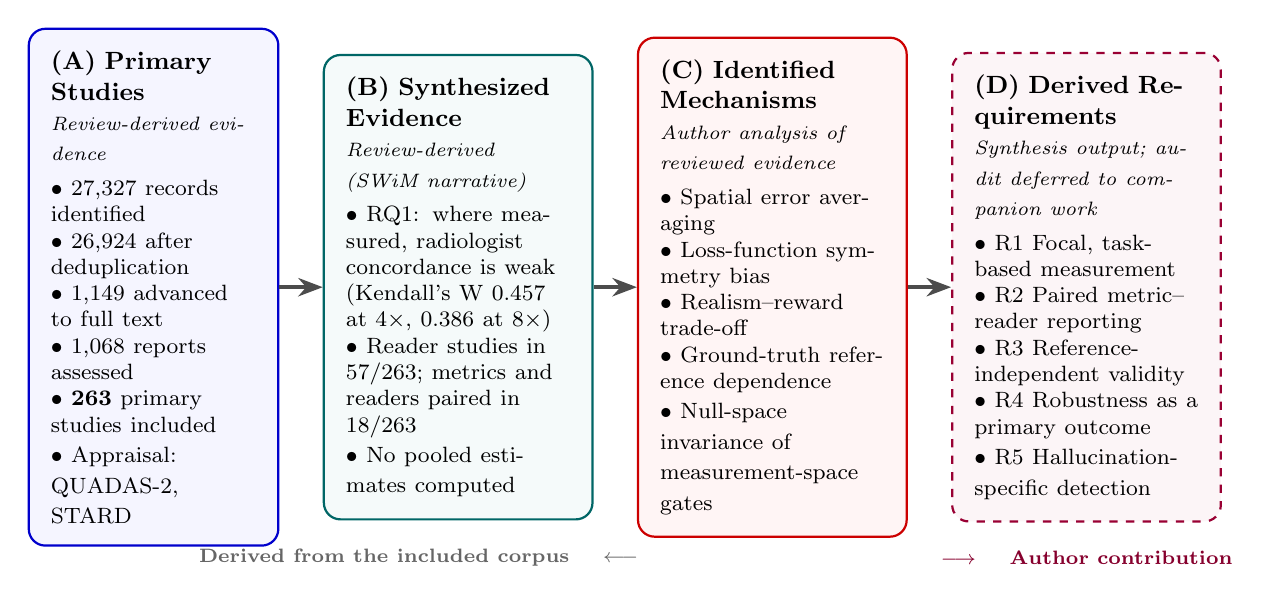
\begin{tikzpicture}[
    node distance=0.7cm and 0.7cm,
    stageA/.style={draw=blue!80!black, rectangle, rounded corners=6pt, fill=blue!4, thick, inner sep=8pt, align=left, font=\small, minimum height=4.6cm},
    stageB/.style={draw=teal!80!black, rectangle, rounded corners=6pt, fill=teal!4, thick, inner sep=8pt, align=left, font=\small, minimum height=4.6cm},
    stageC/.style={draw=red!80!black, rectangle, rounded corners=6pt, fill=red!4, thick, inner sep=8pt, align=left, font=\small, minimum height=4.6cm},
    stageD/.style={draw=purple!80!black, rectangle, rounded corners=6pt, fill=purple!4, thick, inner sep=8pt, align=left, font=\small, minimum height=4.6cm, dashed},
    banner/.style={rectangle, rounded corners=3pt, inner sep=3pt, font=\scriptsize\bfseries},
    arrow/.style={->, >=Stealth, line width=1.3pt, color=black!70}
]

% Stage 1: Primary studies (evidence base)
\node[stageA, text width=0.215\textwidth] (s1) {
    \textbf{(A) Primary Studies}\\
    {\scriptsize\textit{Review-derived evidence}}\\ \vspace{3pt}
    \footnotesize
    $\bullet$ $27{,}327$ records identified\\
    $\bullet$ $26{,}924$ after deduplication\\
    $\bullet$ $1{,}149$ advanced to full text\\
    $\bullet$ $1{,}068$ reports assessed\\
    $\bullet$ $\mathbf{263}$ primary studies included\\
    $\bullet$ Appraisal: QUADAS-2, STARD
};

% Stage 2: Synthesized evidence
\node[stageB, right=0.55cm of s1, text width=0.235\textwidth] (s2) {
    \textbf{(B) Synthesized Evidence}\\
    {\scriptsize\textit{Review-derived (SWiM narrative)}}\\ \vspace{3pt}
    \footnotesize
    $\bullet$ RQ1: where measured, radiologist concordance is weak (Kendall's W $0.457$ at $4\times$, $0.386$ at $8\times$)\\
    $\bullet$ Reader studies in $57/263$; metrics and readers paired in $18/263$\\
    $\bullet$ No pooled estimates computed
};

% Stage 3: Identified mechanisms
\node[stageC, right=0.55cm of s2, text width=0.235\textwidth] (s3) {
    \textbf{(C) Identified Mechanisms}\\
    {\scriptsize\textit{Author analysis of reviewed evidence}}\\ \vspace{3pt}
    \footnotesize
    $\bullet$ Spatial error averaging\\
    $\bullet$ Loss-function symmetry bias\\
    $\bullet$ Realism--reward trade-off\\
    $\bullet$ Ground-truth reference dependence\\
    $\bullet$ Null-space invariance of measurement-space gates
};

% Stage 4: Proposed conceptual framework
\node[stageD, right=0.55cm of s3, text width=0.235\textwidth] (s4) {
    \textbf{(D) Derived Requirements}\\
    {\scriptsize\textit{Synthesis output; audit deferred to companion work}}\\ \vspace{3pt}
    \footnotesize
    $\bullet$ R1 Focal, task-based measurement\\
    $\bullet$ R2 Paired metric--reader reporting\\
    $\bullet$ R3 Reference-independent validity\\
    $\bullet$ R4 Robustness as a primary outcome\\
    $\bullet$ R5 Hallucination-specific detection
};

\draw[arrow] (s1) -- (s2);
\draw[arrow] (s2) -- (s3);
\draw[arrow] (s3) -- (s4);

\node[banner, below=0.25cm of s2.south, xshift=-0.5cm, text=black!60] {Derived from the included corpus \quad $\longleftarrow$};
\node[banner, below=0.25cm of s4.south, text=purple!70!black] {$\longrightarrow$ \quad Author contribution};

\end{tikzpicture}%
}
\caption{Evidence provenance flow for this review, distinguishing what is derived from the included literature from what the authors propose. (A)~PRISMA 2020 selection yields the 263-study evidence base. (B)~Structured narrative synthesis (SWiM) reports findings as representative values from individual primary studies; no statistical pooling was performed. (C)~The four metric-failure mechanisms and the null-space invariance result are the authors' analytical formalization of patterns observed across the reviewed evidence. (D)~The synthesis closes with five derived requirements for safety-oriented evaluation and a prioritized research agenda (the main manuscript); the auditing framework they motivate is developed and evaluated in companion work, not in this review.}
\label{fig:evidence_flow}
\end{figure}


\begin{table}[t]
\centering
\caption{(S13) The post-hoc venue-classification rule as executed, moved here from the main
manuscript. Each study's journal title, and nothing else about the study, is matched
case-insensitively against the three lists \emph{in the order shown}; the ordering is
load-bearing, since a title such as \emph{Medical Image Analysis} matches both the first
and third lists. Anything unmatched is left unclassified rather than forced into a group.
Applied identically to all 263 studies; released as
\texttt{5\_Code/venue\_classification.py}.}
\label{tab:venue_rule}
\small
\begin{tabular}{>{\raggedright\arraybackslash}p{0.26\textwidth} >{\raggedright\arraybackslash}p{0.66\textwidth}}
\hline
\textbf{Group (in order)} & \textbf{Keywords} \\
\hline
1. Engineering and methods & \texttt{ieee}, \texttt{medical image analysis}, \texttt{medical physics}, \texttt{miccai}, \texttt{isbi}, \texttt{arxiv}, \texttt{proceedings}, \texttt{conference}, \texttt{symposium}, \texttt{workshop}, \texttt{pattern recognition}, \texttt{computer methods}, \texttt{computerized medical imaging}, \texttt{physics in medicine}, \texttt{machine learning}, \texttt{signal processing}, \texttt{biomedical engineering}, \texttt{access}, \texttt{sensors}, \texttt{informatics}, \texttt{neural networks} \\
\hline
2. General neuroscience and neuroimaging & \texttt{neuroimage}, \texttt{scientific reports}, \texttt{plos}, \texttt{nature}, \texttt{bmc}, \texttt{frontiers}, \texttt{human brain mapping}, \texttt{elife}, \texttt{communications}, \texttt{heliyon}, \texttt{peerj}, \texttt{neuroinformatics} \\
\hline
3. Clinical imaging & \texttt{radiolog}, \texttt{ajnr}, \texttt{jmri}, \texttt{magnetic resonance in medicine}, \texttt{magnetic resonance imaging}, \texttt{nmr in biomedicine}, \texttt{magma}, \texttt{clinical}, \texttt{tomography}, \texttt{investigative}, \texttt{academic radiology}, \texttt{stroke}, \texttt{neurosurg}, \texttt{medicine}, \texttt{diagnostics}, \texttt{quantitative imaging}, and the national and regional radiology titles listed in the released script \\
\hline
4. Unclassified & no match on any list \\
\hline
\end{tabular}
\end{table}

\begin{table}[t]
\centering
\caption{(S14) Recorded reason for each of the 81 candidate reports whose full text could
not be obtained, moved here from the main manuscript. Every report was checked against its
publisher platform individually. The breakdown bounds what non-retrieval can be hiding; it
does not characterise it, and Section~5.2 of the main manuscript treats the direction of
the resulting bias.}
\label{tab:nonretrieval}
\small
\begin{tabular}{>{\raggedright\arraybackslash}p{0.60\textwidth} r}
\hline
\textbf{Recorded reason} & \textbf{$n$} \\
\hline
Title-level subscription not held, of which: & 53 \\
\quad IOP & 11 \\
\quad Wolters Kluwer & 8 \\
\quad Elsevier society titles & 7 \\
\quad ARRS, SAGE, Karger, RSNA, BMJ, IOS Press, Thieme, Wiley and eight further houses & 27 \\
Springer conference chapters sold per chapter, outside the library agreement & 13 \\
ISMRM proceedings abstracts issued as web pages with no PDF & 4 \\
Citation resolves to a whole proceedings volume or to front matter & 4 \\
No DOI and no source any search could locate & 7 \\
\hline
\textbf{Total} & \textbf{81} \\
\hline
\end{tabular}
\end{table}

\clearpage

\renewcommand{\refname}{References (included studies and supplementary citations)}

\bibliographystyle{elsarticle-num}

\bibliography{ref2}

\end{document}